\documentclass[11pt,a4paper]{article}

% ------------------------------------------------------------
% Packages
% ------------------------------------------------------------
\usepackage[utf8]{inputenc}
\usepackage[T1]{fontenc}
\usepackage{lmodern}
\usepackage[english]{babel}
\usepackage[a4paper,margin=2.5cm]{geometry}
\usepackage{amsmath,amssymb}
\usepackage{siunitx}
\usepackage{booktabs}
\usepackage{array}
\usepackage{graphicx}
\usepackage{float}
\usepackage{caption}
\usepackage{subcaption}
\usepackage{pgfplots}
\usepackage{pgfplotstable}
\usepackage{xcolor}
\usepackage{enumitem}
\usepackage{hyperref}
\usepackage{microtype}
% \usepackage{siunitx}

% ------------------------------------------------------------
% Custom commands
% ------------------------------------------------------------
\newcommand{\degCel}{\,^\circ\mathrm{C}}
\newcommand{\Frac}[2]{\left(\frac{#1}{#2}\right)}
\setlength{\parindent}{0pt}




\pgfplotsset{compat=1.18}

\sisetup{
    per-mode=symbol,
    exponent-product=\cdot,
    output-decimal-marker={.},
    group-separator={,},
    group-minimum-digits=4
}

\hypersetup{
    colorlinks=true,
    linkcolor=black,
    citecolor=black,
    urlcolor=blue,
    pdftitle={Assignment 5 - Generator Design Tool}
}

% ------------------------------------------------------------
%                       Document information
% ------------------------------------------------------------
\title{
    \textbf{FENT2321}\\[0.3cm]
    Wind Energy and Design of a Wind Turbine\\[0.5cm]
    \Large Assignment 6: Reflecting on the generator design
}

\author{Markus Arntzen}
\date{}

\begin{document}

\maketitle
\thispagestyle{empty}

\clearpage
\tableofcontents
\clearpage


% ------------------------------------------------------------
%                       Sections
% ------------------------------------------------------------
\section*{Problem 1: Operating point variables}
\addcontentsline{toc}{section}{Problem 1: Operating point variables}

\setlength{\tabcolsep}{1em}
\renewcommand{\arraystretch}{1.5}
\begin{table}[h]
    \centering
    \begin{tabular}{| l |c|c|}
        \hline
        \textbf{Parameter} & \textbf{Value} & \textbf{Unit} \\
        \hline
        Design RPM & 1420 & RPM \\
        \hline
        Induced voltage at design RPM & 18.9 & V \\
        \hline
        Terminal voltage at design OP & 13.9 & V \\
        \hline
        Output power at design OP & 48.5 & W \\
        \hline
        Efficiency at design OP & 27.4 & \% \\
        \hline
    \end{tabular}
\end{table}

\vspace{1.5cm}

\section*{Problem 2: Changing the active length (Lactive, C26)}
\addcontentsline{toc}{section}{Problem 2: Changing the active length (Lactive, C26)}

\textbf{2 a)} The induced voltage is doubled as the active length is a factor in the formula
for induced voltage, hence doubling the active length equals to multiplying the induced voltage by 2.
\newline

\textbf{2 b)} The stator resistance is increased. This is because the total lenght of wire is increased
as we double the active length of the coils which makes up for a lot of lenght of each coil.
\newline

\textbf{2 c)} Doubling the active coil length means making the part of the coil that is exposed to
the magnetic field twice as long. In practice, the stator/rotor would typically be made longer in
the axial direction.
\newline

\textbf{2 d)} If the "active length" of the magnets doesn't change the length of the coils that are added,
will not experience the same B-field and thus not directly "double" the induced voltage.
Leakage flux will also play a role near the end of the coils.
\newline

\textbf{2 e)} The formula for induced voltage becomes invalid now. We can't just double the active coil length
because that implies that the magnetic field B is uniform and constant over the whole length. In the excel-sheet,
the length of the magnets are stated to be 120mm, and will therefore not reach and supply the same field strength
to the whole coil lengths.

\clearpage

\section*{Problem 3: Changing the number of turns (Nturn, C25)}
\addcontentsline{toc}{section}{Problem 3: Changing the number of turns (Nturn, C25))}

\textbf{3 a)}
\renewcommand{\arraystretch}{1}
\begin{figure}[htbp]
    \centering
    % Table
    \begin{minipage}[t]{0.45\textwidth}
        \centering
        \begin{tabular}{|l|c|}
            \hline
            \textbf{Nturn} & \textbf{Efficiency} \\
            \hline
            20  & 12.8\% \\
            \hline
            30  & 21.0\% \\
            \hline
            40  & 25.1\% \\
            \hline
            50  & 27.6\% \\
            \hline
            60  & 29.3\% \\
            \hline
            70  & 30.4\% \\
            \hline
            80  & 31.3\% \\
            \hline
            90  & 32.0\% \\
            \hline
            100 & 32.6\% \\
            \hline
        \end{tabular}
        \caption{Efficiency for different numbers of turns.}
        \label{tab:efficiency}
    \end{minipage}
    \hfill
    % Picture
    \begin{minipage}[t]{1\textwidth}
        \centering
        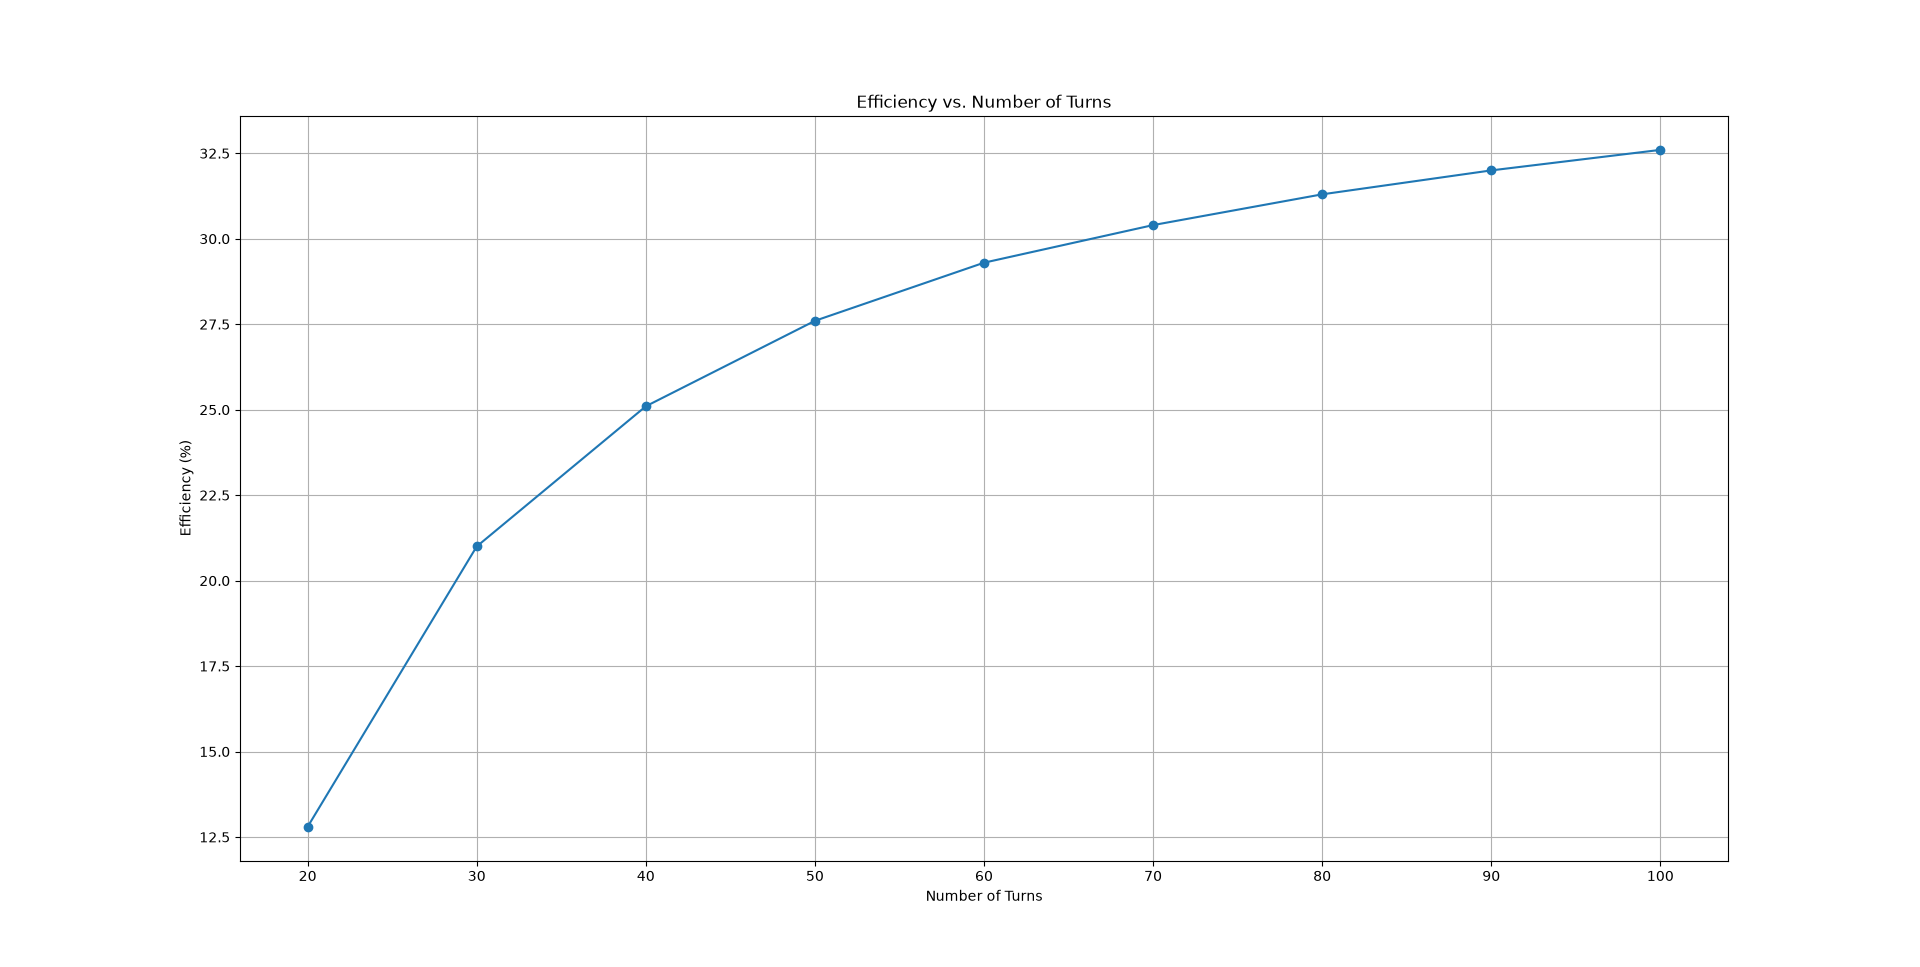
\includegraphics[width=\textwidth]{Figure_1.png}
        \caption{Your figure caption.}
        \label{fig:Plot}
    \end{minipage}
\end{figure}

The efficiency is trending upwards for increased number of turns as is expected, but
we can see the the drop off in efficiency increase which indicates a lower gain for
increased number of turns as we go upwards.
\newline

\textbf{3 b)}
With 100 turns, the coil would contain a large amount of copper wire compared
with the original design. The coil would therefore take up more space and be
more difficult to manufacture and wind. Keeping the same wire diameter also
means that the coil becomes physically larger as more turns are added.
\newline

\textbf{3 c)}
Increasing the number of turns affects several parameters in the Excel sheet.
Two important examples are the stator resistance and the stator inductance.
The stator resistance increases because the total length of copper wire
increases with the number of turns. The stator inductance also increases
strongly because the inductance in the Excel model is proportional to the
square of the number of turns. Therefore, increasing the number of turns
from 50 to 100 increases the inductance by a factor of four.
\newline

\textbf{3 d)}
By increasing to 4 poler and 4 coils in series, in addition to choosing
a copper diameter of 0.00118m, the efficiency initally increases to ~62\%, but
this gives a $T_{diff}$ of about 2Nm. By tuning $R_{load}$, I will not get
to within the boundaries set without going over 50$\Omega$ which is above the
upper boundry set in the excel. If this was possible however, our generator
would be almost double the efficiency for $N_{turn}$ = 100 in a).

\vspace{1.5cm}

\section*{Problem 4: Changing the diameter of the copper wire (Dcu, C24)}
\addcontentsline{toc}{section}{Problem 4: Changing the diameter of the copper wire (Dcu, C24)}

\textbf{4 a)}
When the copper wire diameter is increased to 2.5mm, the cross-sectional area of the copper
wire increases and a larger cross-sectional area gives a lower resistance.
The lower resistance also reduces the copper losses and as a result, less power is lost as
heat in the copper and the efficiency increases. In the excel model, the efficiency
increases from the original value to approximately 41.5\% when the wire diameter is
increased to 2.5mm and the load resistance is adjusted to 17.25$\Omega$ so that the torque
difference becomes < 0.01.
\newline

\textbf{4 b)}
Using thicker copper wire makes each turn physically larger because the wire
occupies more space. This can increase the size of the coil and may require changes to the
coil geometry. The thicker wire also reduces the resistance significantly.
However, the effect on the overall generator geometry depends on whether there is
enough available space for the larger wire. Therefore, using thicker wire can improve
the electrical performance, but it can also create practical manufacturing and
space constraints.

\vspace{2cm}

\section*{PART 2}
\addcontentsline{toc}{section}{PART 2}
\begin{figure}[h]
    \centering
    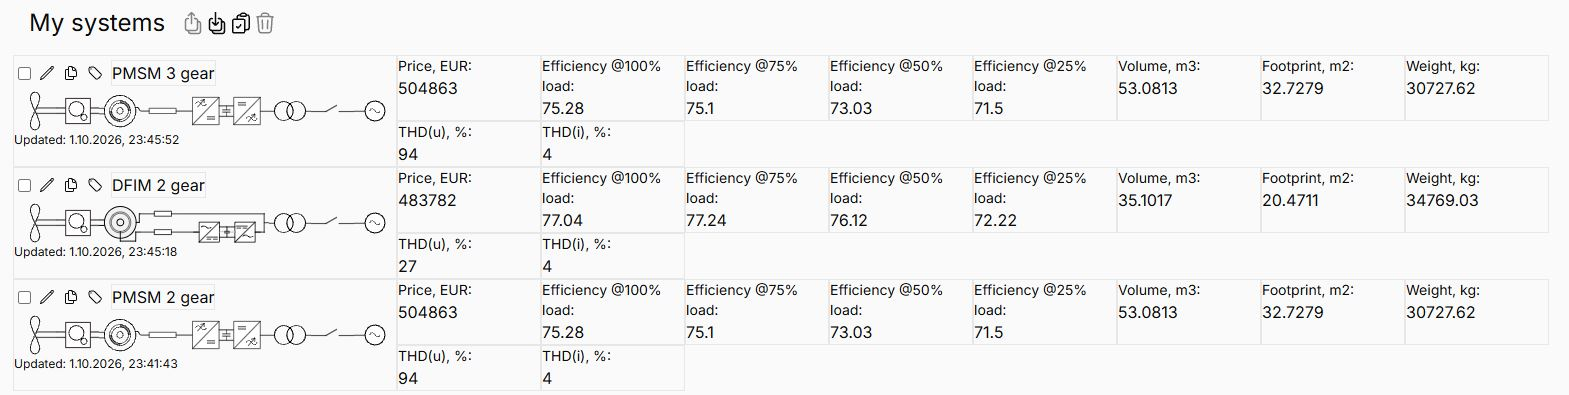
\includegraphics[width=\textwidth]{part2.JPG}
    \caption{Comparison of different drive trains.}
    \label{fig:pmsm_3gear}
\end{figure}

\end{document}